\documentclass[../main/main.tex]{subfiles}
\begin{document}
\raggedbottom

% \dominitoc
% \faketableofcontents
% \dominilof
% \fakelistoffigures
% \dominilot
% \fakelistoftables

\chapter{Supernovae de type Ia}\label{ch:sne}

\epigraph{\openquote\ Il faut porter en soi un chaos pour pouvoir mettre
au monde une étoile dansante.\closequote}{\textsc{Nietzsche}, \textit{Ainsi
parlait Zarathoustra}}

Il existe toute une zoologie d'astres dans l'Univers, entre les planètes, les
étoiles, les galaxies… Ces astres étaient pendant longtemps considérés comme
immuables. Pourtant, en 1572 l'astronome Tycho \textsc{Brahé} vu apparaître une
nouvelle «~étoile~» dans le ciel, et décida donc de la nommer \textit{nova}. Ce
n'est qu'un peu avant le milieu de \textsc{xx}\ieme~siècle que le terme
«~supernova~» fut employé pour la première fois par~\cite{baade1934}, ayant
déterminé que ces objets pouvaient émettre plus de lumière que leur galaxie hôte
sur une courte période de temps.

Au sein des événements caractérisés comme supernovae, il existe des
sous-catégories, dont les SNe~Ia font partie. Nous détaillons dans ce chapitre
ce qui les définit (Section~\ref{sec:death}), quelles sont leurs propriétés
physique d'intérêt (Section~\ref{sec:sneprop}) et comment les utiliser en tant
que chandelles standardisées pour la cosmologie (Section~\ref{sec:stand}).

\vfill
\minitoc
\vfill
\newpage

\section{Fin de vie des étoiles}\label{sec:death}

Si l'existence-même des étoiles est remarquable, la fin de vie de ces réacteurs
nucléaires en puissance l'est au moins tout autant. Nous nous attachons dans
cette section à décrire une fin de vie particulière de ces astres, les
supernovae\footnote{Le pluriel de «~supernova~» est souvent écrit de cette
manière, et se lit «~supernové~».}, et plus particulièrement la sous-catégorie
de celles dites de type «~Ia~»\footnote{Se lit [\textipa{\~EA}].}.

\subsection{Classification}\label{ssec:class} % strolger2004, 2.2

Les supernovae sont le résultat de l'explosion spectaculaire d'une étoile. À cet
effet, ce sont des phénomènes transitoires, c'est-à-dire dont la durée de vie
est courte même à l'échelle humaine~: leur luminosité augmente drastiquement et
diminue jusqu'à revenir à un état pré-explosion sur une durée typique de
quelques semaines. Une première classification par~\cite{minkowski1941} a permis
de distinguer les types I et les types II selon leur composition chimique~: les
premières ne possèdent pas de raie d'hydrogène dans leur spectre\footnote{Mesure
    du flux lumineux selon la longueur d'onde (c'est-à-dire la «~couleur~»)~:
    les éléments chimiques rayonnent ou absorbent des couleurs particulières et
caractéristiques.}, les secondes en ont une. Plus tard, \cite{elias1985}
affinent cette classification en distinguant des sous-types Ia, Ib et Ic,
grâce à l'amélioration des mesures spectrales~: les Ia présentent des raies
de silicium dans leur spectre, les deux autres non et sont séparées selon la
force de leurs raies d'hélium. Cette classification est résumée
Figure~\ref{fig:sne_class}.

\begin{figure}[ht]
    \centering
    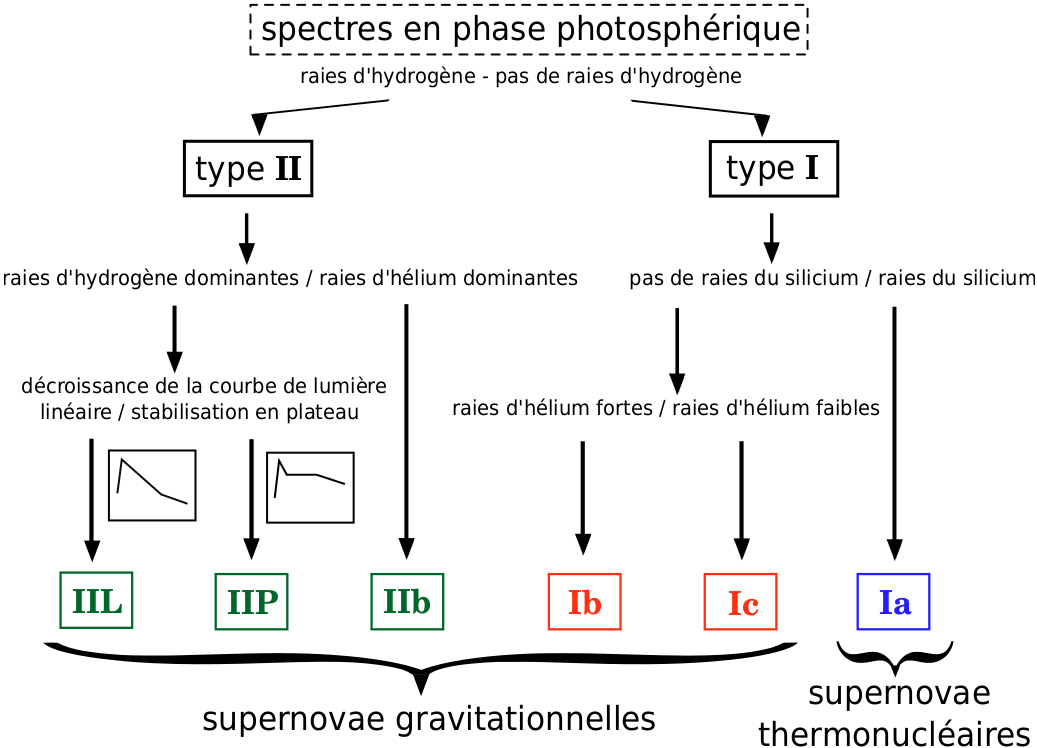
\includegraphics[width=.8\linewidth]{fourmanoit_sne}
    \caption[Classification des différents types de SNe selon leurs
    caractéristiques spectrales]{Classification des différents types de SNe selon
        leurs caractéristiques spectrales. Graphique tiré de la thèse
    de~\cite{fourmanoit2010}.}\label{fig:sne_class}
\end{figure}

Cependant, une différence de taille sépare les SNe~Ia de toutes les autres~:
l'origine et la physique de leur explosion. \cite{filippenko1988} dans un
premier temps et~\cite{heger2003} ensuite déterminent que les SNe non-Ia
résultent de l'effondrement gravitationnel d'une étoile massive, de masse
$M\footnote{Selon le contexte, $M$ peut être soit la magnitude absolue comme
présentée dans le chapitre précédent, soit la masse d'un corps comme ici.} \geq
\SI{8}{\Msun}\footnote{Il est usuel d'exprimer les masses des corps par rapport
à celle du Soleil~: $\Msun = \SI{1.98847\pm0.00007e30}{kg}$.}$~: la fin des
réactions nucléaires exerçant une pression de radiation au cœur de celles-ci ne
compense plus l'attraction gravitationnelle sur les couches externes, qui
s'effondrent au centre avant d'en rebondir en supernova. Elles sont appelées
«~supernovae gravitationnelles~» pour cette raison. Ceci n'est pas possible
pour des étoiles de masses inférieures à \SI{8}{\Msun}, qui vont simplement
perdre leurs couches extérieures pour ne conserver que leurs noyaux
nucléairement inactifs\footnote{Leur équilibre gravitationnel est alors assuré
par la pression de dégénérescence des électrons.}, formant des naines blanches.
Leur masse chute alors à $\approx \SI{1}{\Msun}$, pour un volume typiquement
égal à celui de la Terre\footnote{Si la Terre avait la masse du Soleil, la
    gravité serait $\approx \num{331658}$ fois plus élevée~: ce sont donc des corps
très denses.} et une température entre \SIrange{8000}{14000}{\degreeCelsius}.
\cite{althaus2010} estiment qu'approximativement 97\% des étoiles connaîtront ce
sort (notamment le Soleil, étant donné sa masse). C'est à partir de ce type
d'astre que les SNe~Ia
sont générées, par un mécanisme que nous classifions de «~thermonucléaire~».
Nous allons maintenant parler de la physique de leur explosion.

\subsection{Physique de l'explosion des SNe~Ia}\label{ssec:explo}

Une limitation intrinsèque à la cosmologie et à l'astrophysique est l'absence de
reproduction des expériences en laboratoire, pour des raisons évidentes. Ceci
implique malheureusement que certains phénomènes sont compliqués à décrire avec
certitude~; c'est le cas avec le mécanisme d'explosion des SNe~Ia. Une étude
théorique par~\cite{chandrasekhar1931} sur la pression de dégénérescence impose
une masse critique à une naine blanche (sans rotation), appelée «~limite de
\textsc{Chandrasekhar}~» et placée à $\approx \SI{1.44}{\Msun}$. Au-delà de
celle-ci, l'étoile devient instable et ré-initie des réactions thermonucléaires,
amorçant la fusion du carbone et de l'oxygène sans régulation, amenant à son
explosion et la désintégrant en totalité.

Si cette partie de la physique de l'explosion est bien admise, la manière dont
une naine blanche augmente sa masse pour dépasser cette limite est encore
débattue. Plusieurs scénarios sont proposés, mais les deux principalement
acceptés sont~:
\paragraph*{Le scénario simplement dégénéré\!\!} \citep{whelan1973} dans lequel la
naine blanche est dans un système binaire avec une étoile compagnon qui va
perdre de sa matière externe au profit de la première~;
\paragraph*{Le scénario doublement dégénéré\!\!} \citep{webbink1984} dans lequel
la naine blanche est dans un système binaire avec une autre naine blanche. Leurs
noyaux durs ne permettant pas de perdre de masse gazeuse, les deux étoiles sont
dans une orbite de plus en plus resserrée en perdant de l'énergie sous forme
d'ondes gravitationnelles\footnote{La propagation d'une déformation de la
métrique même de l'espace-temps, voir Chapitre~\ref{ch:cosmo}.} et finissent par
fusionner si l'une ne se disloque pas sous l'effet de marée de l'autre.

Malheureusement, aucun de ces scénarios n'a pu être privilégié puisqu'ils sont
très difficiles à observer et que les simulations ne sont pas en mesure de
reproduire les observations~\citep{ropke2012}. Ainsi, des modèles empiriques de
l'évolution du spectre des SNe~Ia sont utilisés pour les
caractériser\footnote{Nous les appelons «~distributions spectrales en énergie~»
ou \textit{Spectral Energy Distribution} (SED) en anglais.} (voir
Section~\ref{ssec:salt}). Il reste qu'en pratique nous observons une remarquable
homogénéité du pic de luminosité de ces explosions, respectant la masse critique
impliquant une quantité d'énergie définie disponible pour l'explosion. C'est de
cette manière qu'elle sont utilisées en tant que chandelles standard, comme
expliqué Section~\ref{ssec:intsne}.

\section{Propriétés}\label{sec:sneprop}

Si leur nature reste imprécise, nous avons observé de nombreuses SNe~Ia. Ces
observations reposent sur leur analyse photométrique (Section~\ref{ssec:lc})
ainsi que sur leurs caractéristiques spectroscopiques
(Section~\ref{ssec:spectro}).

\subsection{Courbe de lumière}\label{ssec:lc}

Comme introduit Section~\ref{ssec:class}, les SNe~Ia sont des phénomènes
transitoires. Ainsi, leur observation par une caméra relève une augmentation de
leur luminosité jusqu'à un pic avant de redescendre~: une telle courbe s'appelle
«~courbe de lumière~». Nous en donnons un exemple
Figure~\ref{fig:2011fe_phot}\footnote{Nous remarquerons que l'échelle verticale
    est inversée étant donné que les magnitudes vont dans le sens opposé à la
luminosité.}.

\begin{figure}[]
    \centering
    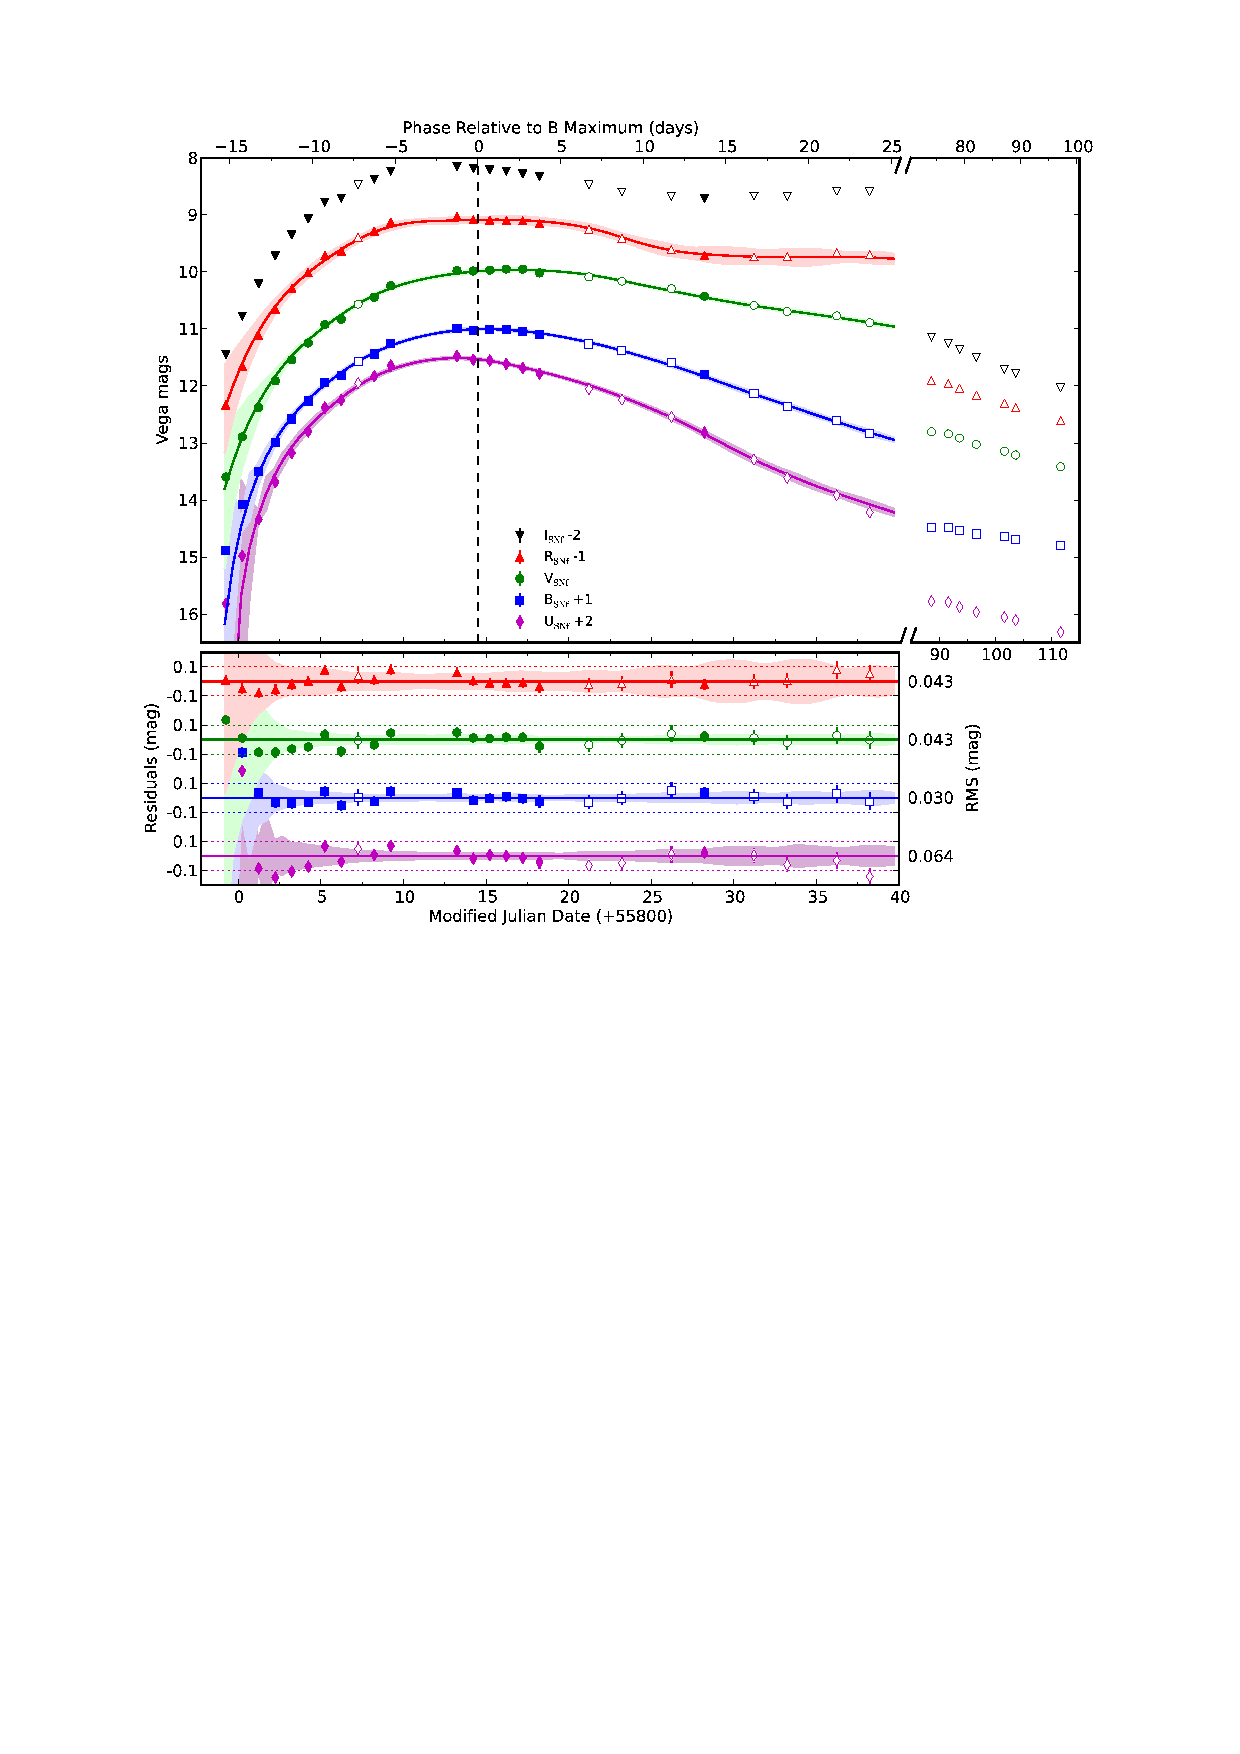
\includegraphics[width=\linewidth,
                     trim={2cm 18.75cm 2.5cm 2.0cm},
                     clip]{2011fe_lightcurves}
    \caption[Courbe de lumière de la SN~Ia SN2011fe]{Courbe de lumière en bandes
        $UBVRI$ de la SN~Ia confirmée SN2011fe avec ajustement par
        \texttt{SALT2} (ligne pleine et bande pour son erreur~;
        voir Section~\ref{ssec:salt}). Figure
    de~\cite{pereira2013}.}\label{fig:2011fe_phot}
\end{figure}

Ces observations s'effectuent non seulement dans le temps mais également pour
différentes couleurs\footnote{Moyenne du flux sur une plage de longueurs
d'ondes, que nous appelons «~bandes photométriques~».}. La diminution de magnitude
est typiquement de \SIrange{3}{6}{mag} sur une quinzaine de jours, que la SN~Ia
regagne ensuite sur une période de plusieurs dizaines de jours ($\approx
\SI{50}{jours}$). À partir de cette courbe se définissent plusieurs
caractéristiques~:

\begin{itemize}
    \item[$t_0$]: date du maximum d'émission dans la bande bleue~;
    \item[$x_0$]: amplitude dans la bande bleue (nous définissons $m_B =
        -2,5\log(x_0)$)~;
    \item[$x_1$]: étirement typique de la courbe de lumière, lié à la largeur de
        la courbe et caractérisant la vitesse de l'explosion (petit $x_1
        \Rightarrow$ explosion rapide)~;
    \item[$c$]: couleur globale de la SN, correspondant à la différence de
        magnitude entre deux bandes~: à bas redshift les bandes bleues
        et vertes sont utilisées (nous écrivons $c = B - V$), mais avec le
        décalage vers le rouge elle peut être estimée différemment.
\end{itemize}

\subsection{Spectroscopie}\label{ssec:spectro}

En plus d'étudier la magnitude d'une SN dans le temps, nous pouvons étudier sa
distribution énergétique en fonction de la longueur d'onde dans le temps, ce
que nous appelons une distribution spectrale ou série spectro-temporelle. Nous
présentons Figure~\ref{fig:2011fe_spec} la série de la SN~Ia SN2011fe.

\begin{figure}[]
    \centering
    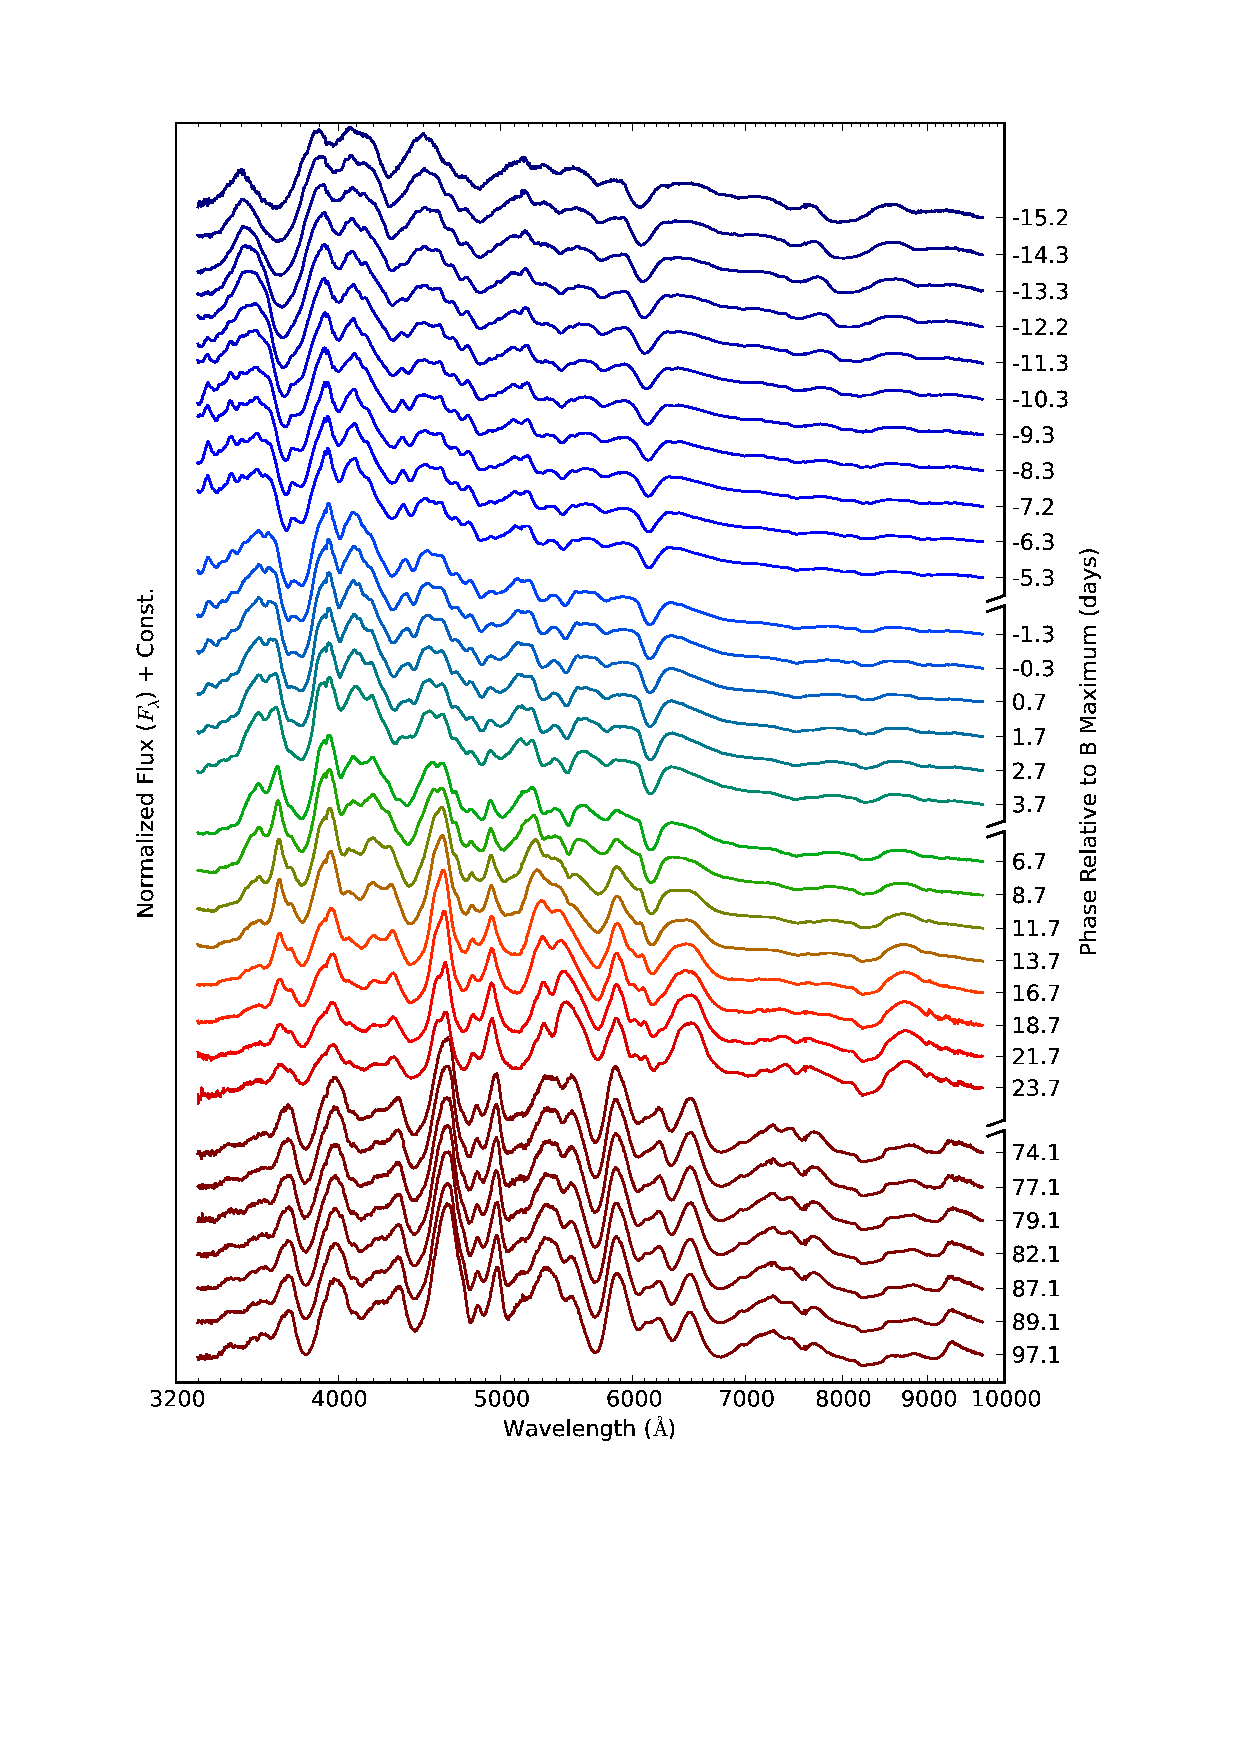
\includegraphics[width=\linewidth,
                     trim={2cm 5cm 2cm 2.0cm},
                     clip]{2011fe_spectro}
    \caption[Série spectro-temporelle de la SN~Ia SN2011fe]{Série
        spectro-temporelle de la SN~Ia SN2011fe entre -15 et \SI{100}{jours} par
        rapport à son maximum d'émission en bande bleue $t_0$. La variation dans
        la profondeur des pics montre l'évolution de la composition chimique de
        la supernova~: désintégration $\prescript{56}{}{\mathrm{Ni}}
        \rightarrow \prescript{56}{}{\mathrm{Co}}$ sur les 15 premiers jours,
        puis $ \prescript{56}{}{\mathrm{Co}} \rightarrow
        \prescript{56}{}{\mathrm{Fe}}$ ensuite. Figure de~\cite{pereira2013}.}
        \label{fig:2011fe_spec}
\end{figure}

L'étude spectrale est plus riche en informations que l'étude photométrique, et
c'est grâce à ces données que le type d'une SN est déterminé. Nous pouvons en
effet déterminer sa composition chimique ainsi que l'évolution de celle-ci
\textit{via} la profondeur des raies d'absorption spécifiques à ces éléments
(raie prononcée $\Rightarrow$ élément en grande proportion). Sur les quinze
premiers jours, la désintégration thermonucléaire d'une SN~Ia est typiquement
dominée par la désintégration $\prescript{56}{}{\mathrm{Ni}} \rightarrow
\prescript{56}{}{\mathrm{Co}}$, avant d'être dominée par 
$\prescript{56}{}{\mathrm{Co}} \rightarrow \prescript{56}{}{\mathrm{Fe}}$
ensuite. De plus, les points photométriques sont des moyennes du flux lumineux
sur certaines plages de longueurs d'ondes, ce qui permet de reconstruire la
courbe de lumière.

C'est également avec la spectroscopie que nous pouvons le plus précisément
estimer le redshift d'un corps (appelé alors «~redshift spectroscopique~»),
étant donné qu'il correspond littéralement à un décalage des longueurs d'ondes
vers le rouge. Cependant, pour n'avoir que le redshift cosmologique dû à
l'expansion de l'Univers et non celui du mouvement propre d'une SN, nous
observons généralement les galaxies hôtes. Outre cet avantage de mouvement
propre, elles présentent des raies plus fines donnant une estimation du redshift
plus précise (précision à $\approx \num{1e-5}$ pour les galaxies contre $\approx
\num{1e-3}$ pour un redshift estimé sur le spectre d'une SN), et n'étant pas des
objets transitoires elles donnent plus de temps pour effectuer la mesure. Ces
trois éléments sont primordiaux pour avoir la meilleure estimation de la
distance de luminosité (qui s'obtient à partir du redshift d'après
l'Équation~\ref{eq:dl}). Si le redshift de l'hôte vient à manquer, nous
l'estimons avec le spectre de la SN directement~; dans le pire des cas il est
estimé à partir de la photométrie de l'hôte.

\subsection{Modèle \texttt{SALT2.4}}\label{ssec:salt}

La détermination précise des paramètres d'une supernova est effectuée en
ajustant un modèle d'évolution spectrale sur les données récoltées. Dans notre
thèse, nous utilisons la version 2.4 du modèle \textit{Spectral Adaptative
Light-curve Template 2} \citep[\texttt{SALT2},][]{guy2007} décrivant l'évolution
de la SED d'une SN~Ia au cours du temps. Cette version a été entraînée sur les
données empiriques de~\cite{betoule2014}. Dans ce modèle, le flux observé $F$
est décrit à un temps $t$ caractérisé par sa phase $p$ (temps par rapport à
$t_0$) et à une longueur d'onde $\lambda$ par~:
\begin{equation}\label{eq:saltf}
    F(p,\lambda) = x_0\left[ M_0(p,\lambda) + x_1M_1(p,\lambda)
    \right]\times \exp(c\cdot CL(\lambda))
\end{equation}
Ici, $M_0$ est la séquence spectrale moyenne, $M_1$ la déviation au premier
ordre autour de cette séquence et $CL$ une loi de couleur. Ce sont des
propriétés globales du modèle~; les paramètres $x_0$, $x_1$ et $c$ sont
spécifiques à une SN, comme nous l'avons vu Section~\ref{ssec:lc}. C'est avec ce
modèle que sont ajustées les courbes de la Figure~\ref{fig:2011fe_phot} et que
sont extraites les valeurs des paramètres.

\section{Standardisation}\label{sec:stand}

En calibrant les distances des SNe~Ia avec d'autres sondes, il est possible de
mesurer leur magnitude absolue. Comme nous l'avons présenté précédemment, nous
la trouvons à une valeur relativement stable, avec $M_0 =
-\SI{19.36}{mag}$~\citep{kessler2009b}, ce qui leur a valu le terme de
«~chandelles standard~». Seulement, il existe une variabilité intrinsèque de
$\approx \SI{0.35}{mag}$ qui amène à une incertitude finale sur la distance
proche de 20\%, ce qui ne permet pas leur utilisation rigoureuse. Pour remédier
à ce problème, il a fallu trouver un moyen de réduire cette variation~: nous
appelons cela la «~standardisation~».

\subsection{Corrélations}\label{ssec:corr}

Par l'étude de la dépendance de la magnitude absolue des SNe~Ia avec leur
étirement $x_1$ et leur couleur $c$, nous pouvons observer une dépendance
avec chacun de ces paramètres. Nous présentons Figure~\ref{fig:mxc} l'évolution
des courbes de magnitude absolues des données de la collaboration \textit{Joint
Light-curve Analysis}~\citep[JLA,][]{betoule2014} en fonction de ces deux
paramètres ainsi que les corrélations observées.

\begin{figure}[]
    \centering
    \begin{subfigure}[c]{.48\linewidth}
        \centering
        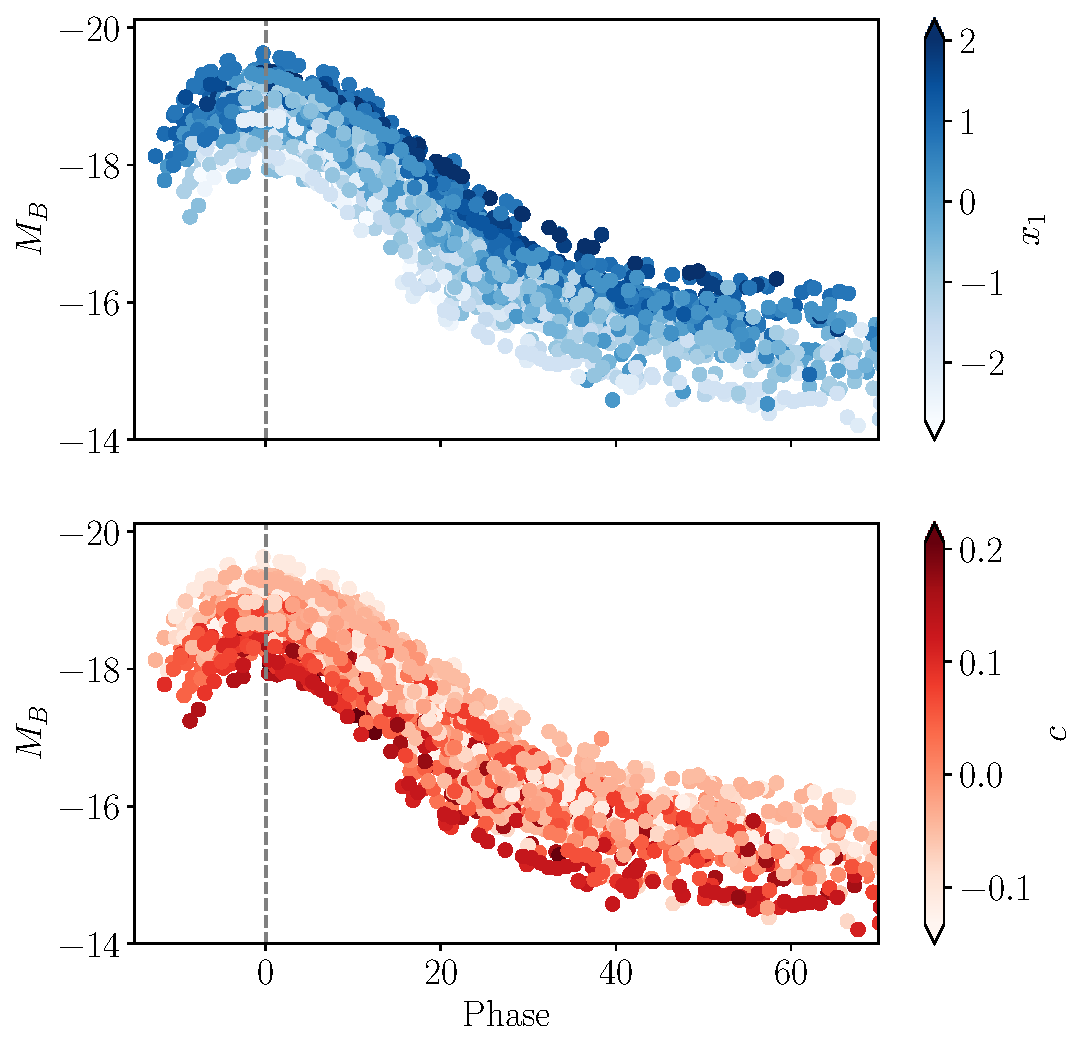
\includegraphics[width=\linewidth]{lc_JLA_nora}
        %\caption{M87}
        \label{fig:mxca}
    \end{subfigure}
    \begin{subfigure}[c]{.48\linewidth}
        \centering
        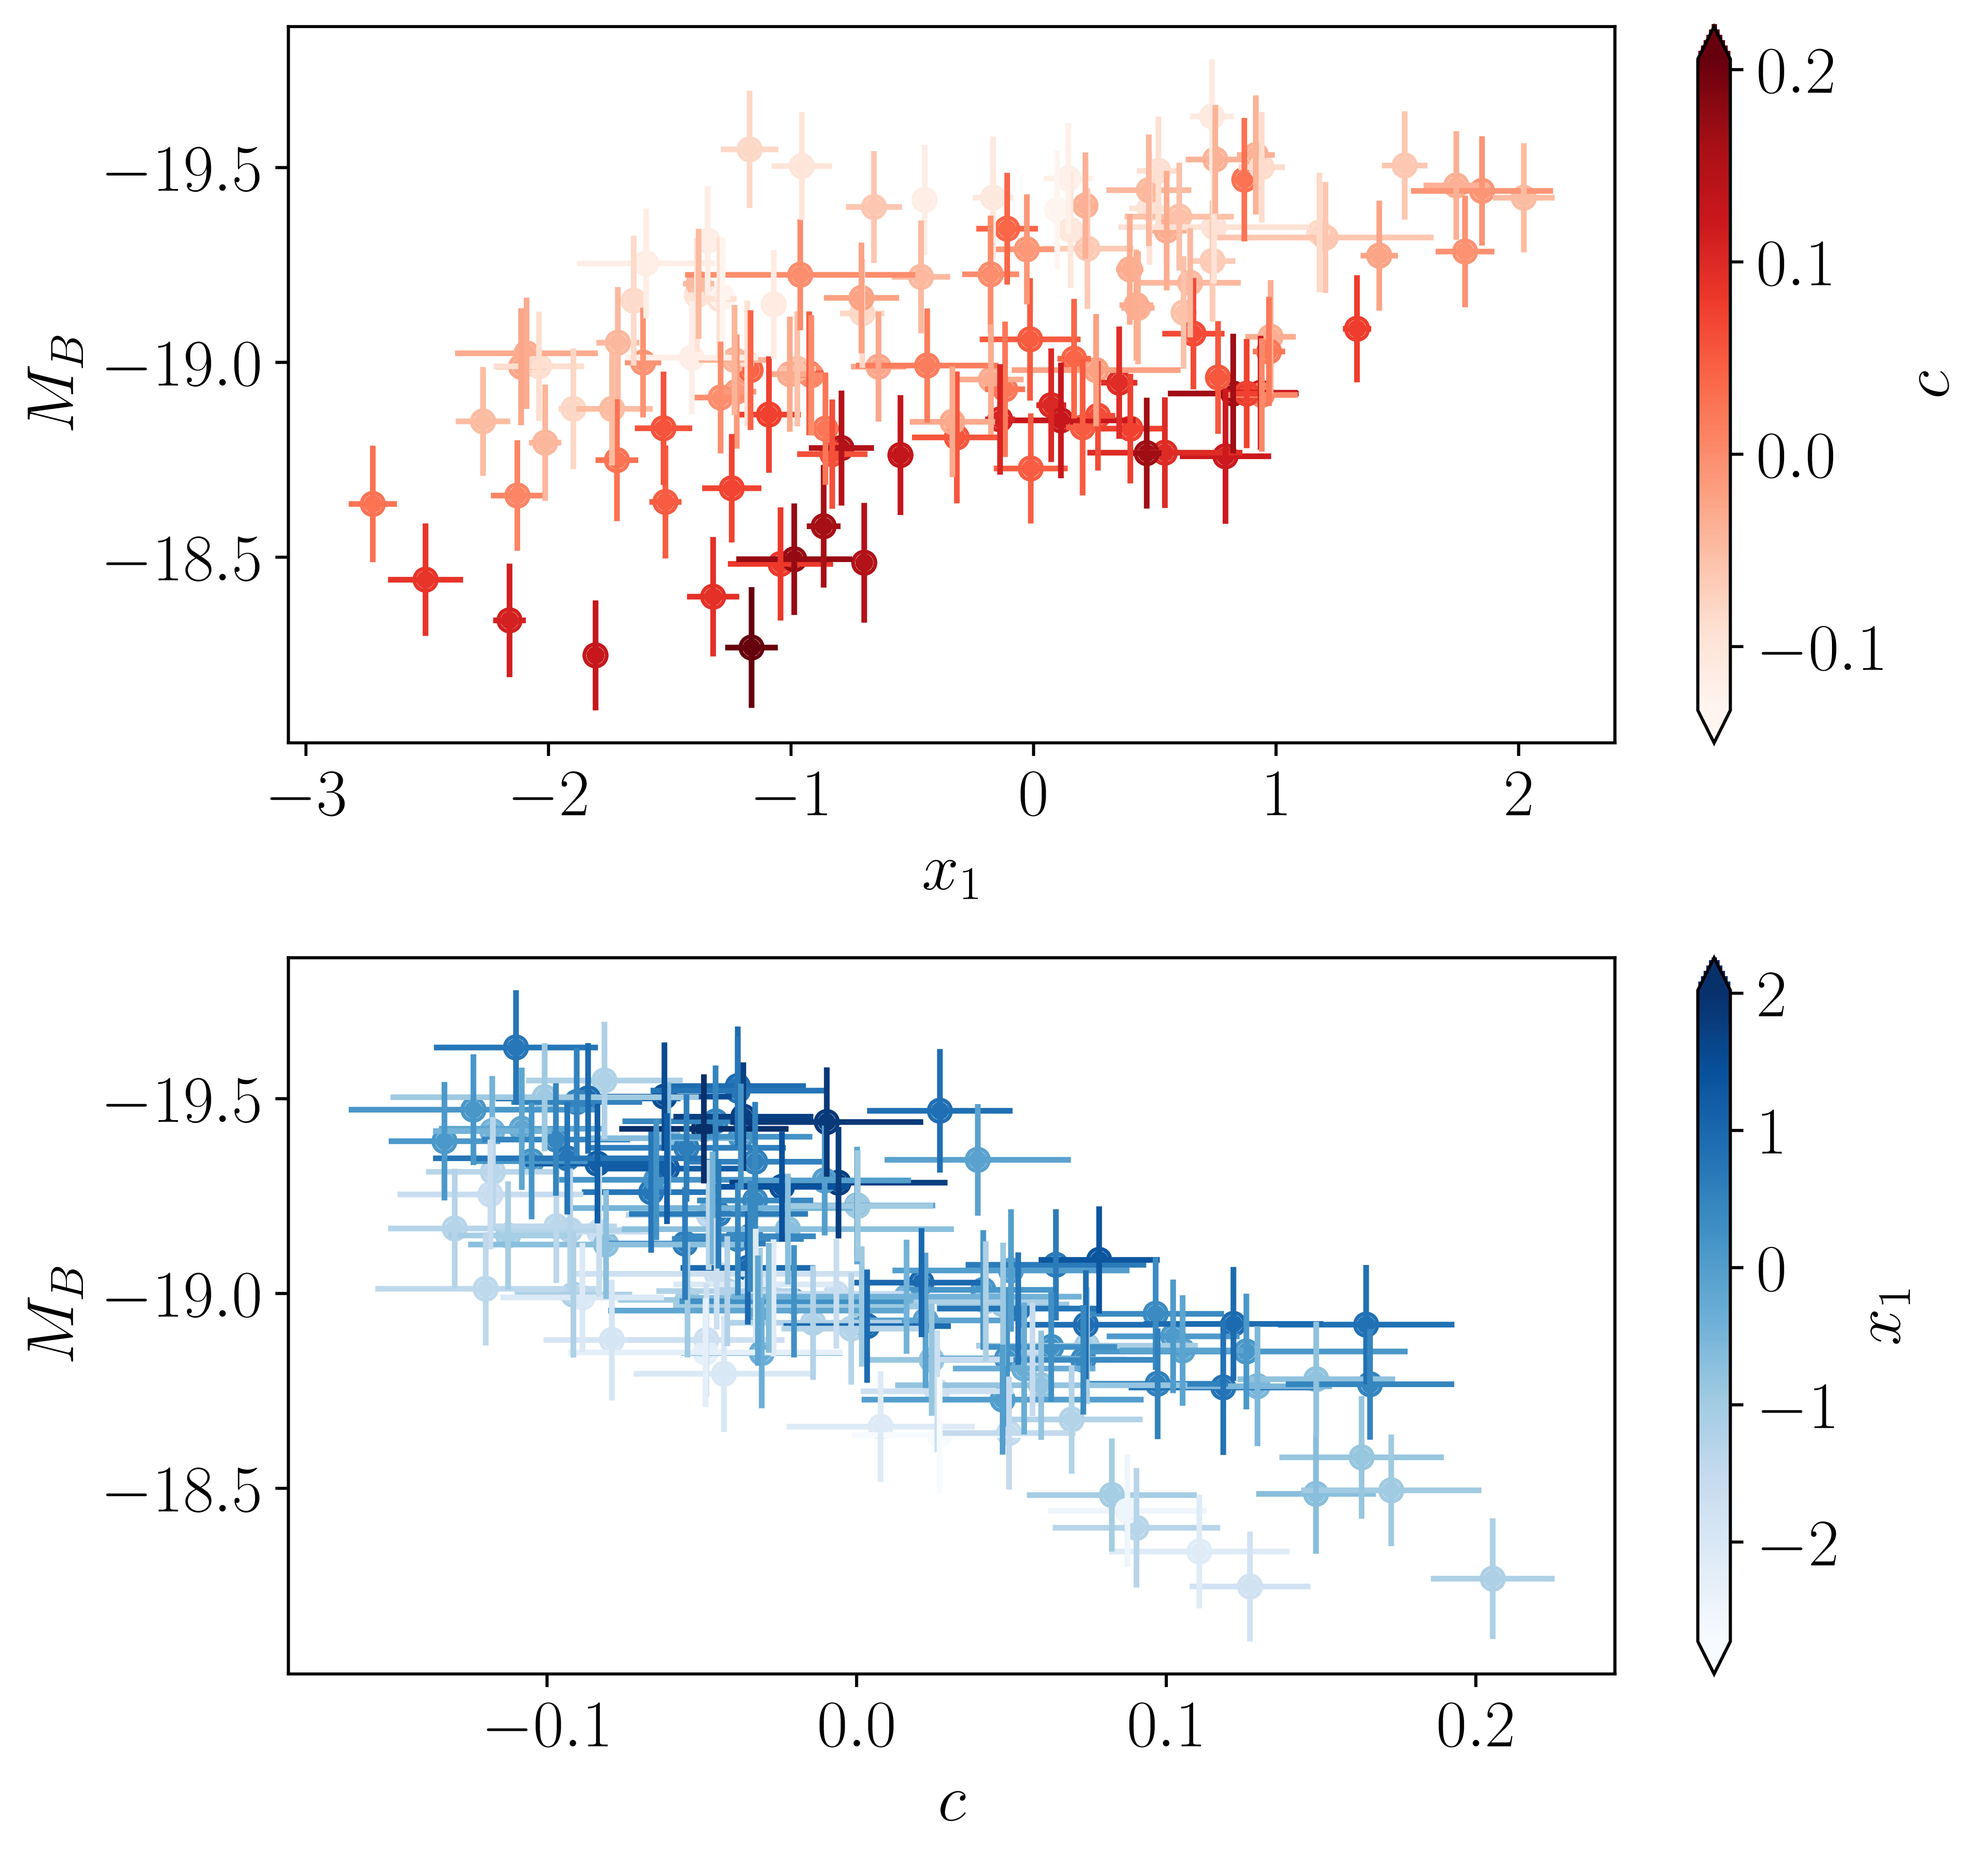
\includegraphics[width=\linewidth]{colorstretch_corr_JLA_nora}
        %\caption{M87}
        \label{fig:mxcb}
    \end{subfigure}
    \caption[Dépendance de la magnitude absolue des SNe~Ia de la collaboration
    JLA avec l'étirement et la couleur]{Dépendance de la magnitude absolue des
        SNe~Ia de la collaboration JLA~\citep{betoule2014} avec l'étirement
        (\textit{en bleu}) et la couleur (\textit{en rouge}). \textit{À
        gauche}~: résultat brut. \textit{À droite}~: corrélations linéaires. La
        relation avec $x_1$ est caractérisée par un coefficient $\alpha$, et
    celle avec $c$ par un coefficient $\beta$.}\label{fig:mxc}
\end{figure}

\cite{phillips1993} a montré en premier lieu l'effet avec l'étirement, qui
montre que les SNe~Ia de grand étirement (évolution lente) sont intrinsèquement
plus lumineuses\footnote{Nous appelons cette corrélation
\textit{slower-brighter} en anglais.}. Cette corrélation linéaire est
caractérisée par un coefficient $\alpha$. Ensuite, \cite{hamuy1996} ont montré
la dépendance avec la couleur~: les SNe~Ia les plus bleues sont plus
lumineuses\footnote{Nous appelons cette corrélation \textit{bluer-brighter} en
anglais.}, relation caractérisée par le coefficient $\beta$. Ces corrélations
sont utilisées pour réduire l'incertitude sur la magnitude absolue selon~:
\begin{equation}\label{eq:mxc}
    M_B = M_0 - \alpha x_1 + \beta c
\end{equation}
Cette relation réduit l'incertitude sur $M_B$ à \SI{0.15}{mag}, et permet
d'établir la relation de~\cite{tripp1998}~:
\begin{equation}
    \mu = m_B - M_B + \alpha x_1 - \beta c
\end{equation}
ce qui amène à $\approx$ 8\% d'incertitude sur la distance.

\subsection{SNe~Ia aujourd'hui}\label{ssec:snetoday}

De cette manière, les SNe~Ia ont pu être utilisées pour découvrir l'expansion
accélérée de l'Univers, comme discuté dans le chapitre précédent. Elles
continuent d'être au cœur de la cosmologie actuelle. Nous présentons
Figure~\ref{fig:hubdiag} le diagramme de \textsc{Hubble} avec les données
de~\cite{scolnic2018} utilisant des SNe~Ia observées par différents sondages
(nous les détaillons Chapitre~\ref{ch:surveys}) formant un échantillon nommé
\textit{Pantheon}.

Au départ, une incertitude systématique\footnote{Qui est systématiquement
présente~; due à la physique intrinsèque des SNe~Ia.} de 8\% était suffisante
pour discriminer des modèles cosmologiques très différents étant donné que les
incertitudes statistiques\footnote{Issues du nombre de points de mesure.}
étaient elles-mêmes dominantes. Seulement, cela devient de moins en moins vrai
au fur et à mesure que les incertitudes statistiques diminuent grâce à la
quantité de données recueillies par différents télescopes. Si nous voulons
mesurer précisément les paramètres cosmologiques aujourd'hui, il devient
nécessaire d'améliorer notre connaissance physique des SNe~Ia, et notamment la
manière de les standardiser. Il existe plusieurs manières de s'intéresser à
cela~; certaines études se concentrent sur de nouveaux modèles spectraux avec
plus de paramètres~\cite[par exemple][]{leget2020}, mais la plupart cherche des
paramètres de standardisation qui soient extérieurs aux SNe~Ia. Nous proposons
dans le chapitre suivant un aperçu des environnements des SNe~Ia et la manière
dont ils sont utilisés pour la cosmologie moderne. Ce chapitre viendra motiver
l'étude précise de notre thèse.

\vfill
\begin{figure}[h]
    \centering
    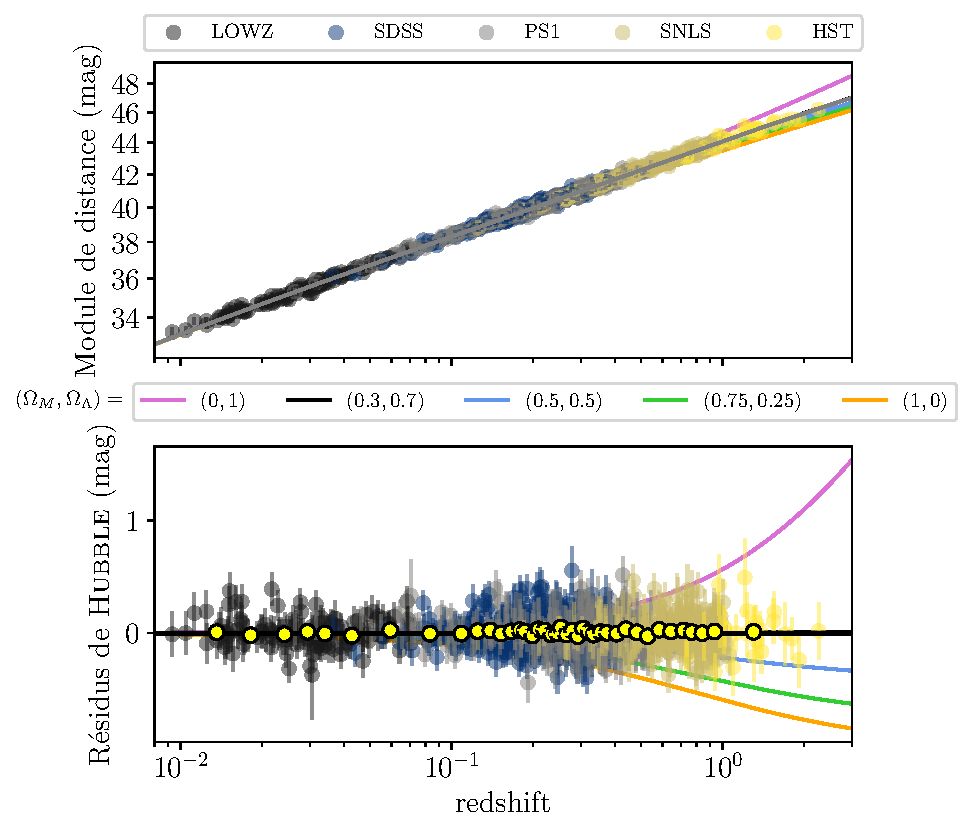
\includegraphics[width=\linewidth]{hd_panth}
    \caption[Diagramme de \textsc{Hubble} avec les données de l'analyse
    Pantheon]{Diagramme de \textsc{Hubble} avec les données de l'analyse
        Pantheon~\citep{scolnic2018}. Figure reproduite. Nous indiquons en
        couleur les modules de distance attendus selon la composition
        énergétique de l'Univers~: nous illustrons ici comment les SNe~Ia
    permettent de contraindre la physique du cosmos.}\label{fig:hubdiag}
\end{figure}
\vfill

\newpage

\thispagestyle{plain}
\vspace*{\fill}
\minilof
\vspace*{\fill}

% \bibliographystyle{../main/aa_url}
% \shorthandoff{:}
% \bibliography{../chapters/99_references}

\end{document}
